\begin{activity} \label{A:3.2.1}  Consider the family of functions defined by $p(x) = x^3 - ax$, where $a \ne 0$ is an arbitrary constant.
	\ba
	\item Find $p'(x)$ and determine the critical values of $p$.  How many critical values does $p$ have? 
	\item Construct a first derivative sign chart for $p$.  What can you say about the overall behavior of $p$ if the constant $a$ is positive?  Why?  What if the constant $a$ is negative? In each case, describe the relative extremes of $p$.
	\item Find $p''(x)$ and construct a second derivative sign chart for $p$.  What does this tell you about the concavity of $p$?  What role does $a$ play in determining the concavity of $p$?
	\item Without using a graphing utility, sketch and label typical graphs of $p(x)$ for the cases where $a > 0$ and $a < 0$.  Label all inflection points and local extrema.	
  	\item Finally, use a graphing utility to test your observations above by entering and plotting the function $p(x) = x^3 - ax$ for at least four different values of $a$.  Write several sentences to describe your overall conclusions about how the behavior of $p$ depends on $a$.
	\ea
\end{activity}
\begin{smallhint}
	\ba
	\item When solving $p'(x) = 0$, think about two possible cases: when $a > 0$ and when $a < 0$.
	\item Remember that any quadratic function can be zero at most two times.  How does the graph of $y = 3x^2 - a$ look?
	\item Don't forget that $\frac{d}{dx}[a] = 0$.
	\item Think about how a typical cubic polynomial's graph behaves.	
	\ea
\end{smallhint}
\begin{bighint}
	\ba
	\item Note that $p'(x) = 3x^2 - a$.  When solving $p'(x) = 0$, think about two possible cases: when $a > 0$ and when $a < 0$.
	\item Remember that any quadratic function can be zero at most two times.  How does the graph of $y = 3x^2 - a$ look?
	\item Don't forget that $\frac{d}{dx}[a] = 0$.
	\item Think about how a typical cubic polynomial's graph behaves and use your work in (a) - (c).	
	\ea
\end{bighint}
\begin{activitySolution}
\ba
  \item We first note that $p'(x) = 3x^2 - a$, so to find critical values we set $p'(x) = 0$ and solve for $x$.  This leads to the equation $3x^2 - a = 0$, which implies 
  $$x^2 = \frac{a}{3}.$$
  If $a > 0$, then the solutions to this equation are $x = \pm \sqrt{\frac{a}{3}}$; if $a < 0$, then the equation has no solution.  Hence, $p$ has two critical numbers ($x = \pm \sqrt{\frac{a}{3}}$) whenever $a > 0$ and no critical numbers when $a < 0$.
  \item For the case when $a < 0$, we observe that $p'(x) = 3x^2 - a$ is positive for every value of $x$, and thus $p$ is always increasing and has no relative extreme values.  (There are no critical numbers to place on the first derivative sign chart, and $p'$ is always positive.)
  
  For the case when $a > 0$, we observe that $p'(x) = 3x^2 - a$ is a concave up parabola with zeros at $x = -\sqrt{\frac{a}{3}}$ and $x = +\sqrt{\frac{a}{3}}$.  It follows that for $x < -\sqrt{\frac{a}{3}}$, $p'(x) > 0$ (so $p$ is increasing); for $-\sqrt{\frac{a}{3}} < x < \sqrt{\frac{a}{3}}$, $p'(x) > 0$ (so $p$ is decreasing); and for $x > \sqrt{\frac{a}{3}}$, $p'(x) > 0$ (so $p$ is again increasing).  In this situation, we see that $p$ has a relative maximum at $x = -\sqrt{\frac{a}{3}}$ and a relative minimum at $x = +\sqrt{\frac{a}{3}}$.
  \item Since $p'(x) = 3x^2 - a$ and $a$ is constant, it follows that $p''(x) = 6x$.  Note that $p''(x) = 0$ when $x = 0$ and that $p''(x) < 0$ for $x < 0$ and $p''(x) > 0$ for $x > 0$.  Hence $p$ is CCD for $x < 0$ and $p$ is CCU for $x > 0$, making $x = 0$ an inflection point.
  \item Below, we show the two possible situations. At left, for the case when $a < 0$ and $p$ is always increasing with an inflection point at $x = 0$, and at right for when $a > 0$ and $p$ has a relative maximum at $x = -\sqrt{\frac{a}{3}}$ and a relative minimum at $x = +\sqrt{\frac{a}{3}}$, again with an inflection point at $x = 0$.  Note, too, that $p$ has its $x$-intercepts at $x = \pm \sqrt{a}$.
  \begin{center}
  	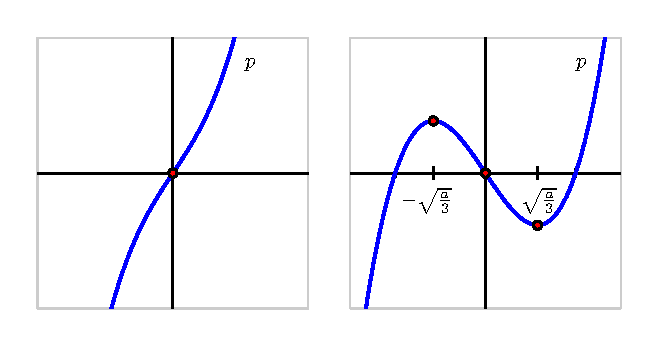
\includegraphics{figures/3_2_Act1Soln.eps}
  \end{center}
\ea
\end{activitySolution}
\aftera